%
%
% -------------------------------------------------
%
\documentclass[11pt, a4paper]{amsart}
%
%
%
\usepackage[latin1]{inputenc}
\usepackage[english]{babel}
\selectlanguage{english}
%
\usepackage{hyperref}
\usepackage[twoside=false]{geometry}
% \usepackage{cmbright}
\usepackage{bm}
\usepackage{cleveref}
\usepackage{xparse}
\usepackage[textsize=footnotesize]{todonotes}
\usepackage{subfigure}
\usepackage{float}
%
%
%
\title{Sensor Fusion Midterm Project}
\author{Hans Franzen}
\date{}
%
%
% ----------------------------------------------------------------------------------------------------
%
%
\begin{document}

	\maketitle
	
	The following images show several cars in the point cloud images. 
	\begin{figure}[H]
		\centering
		\subfigure[Frame 4]{%
		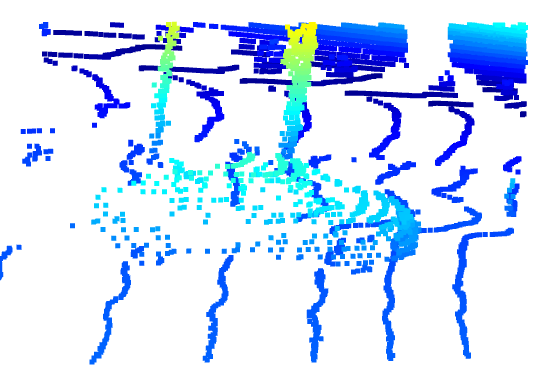
\includegraphics[scale=0.4]{../images_output/Seq1_Frame4.png}}
		\label{S1F4}
		\quad
		\subfigure[Frame 25]{%
		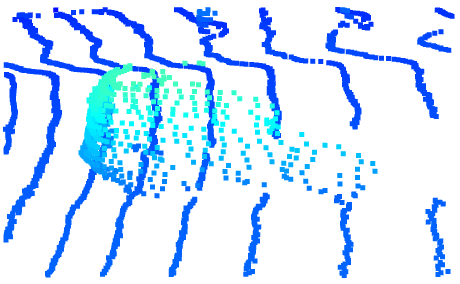
\includegraphics[scale=0.4]{../images_output/Seq1_Frame25.png}}
		\label{S1F25}
		\quad
		\subfigure[Frame 41]{%
		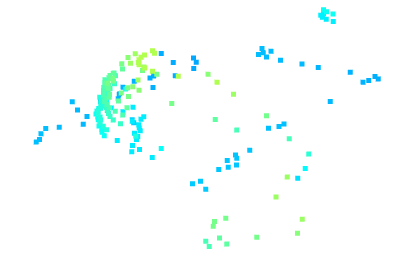
\includegraphics[scale=0.4]{../images_output/Seq1_Frame41.png}}
		\label{S1F41}
		\\
		\subfigure[Frame 60]{%
		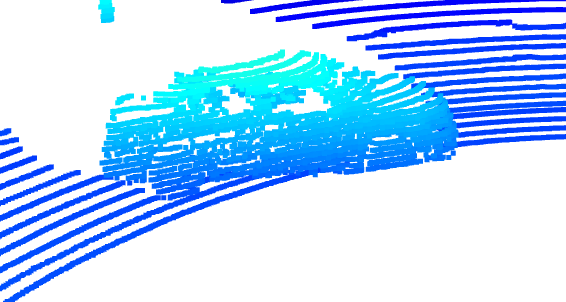
\includegraphics[scale=0.4]{../images_output/Seq1_Frame60.png}}
		\label{S1F60}
		\quad
		\subfigure[Frame 70]{%
		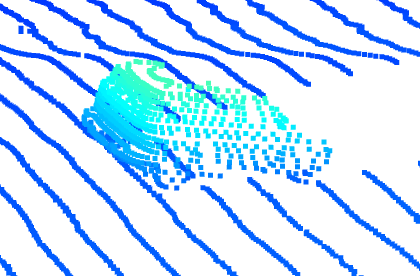
\includegraphics[scale=0.4]{../images_output/Seq1_Frame70.png}}
		\label{S1F70}
		\quad
		\subfigure[Frame 83]{%
		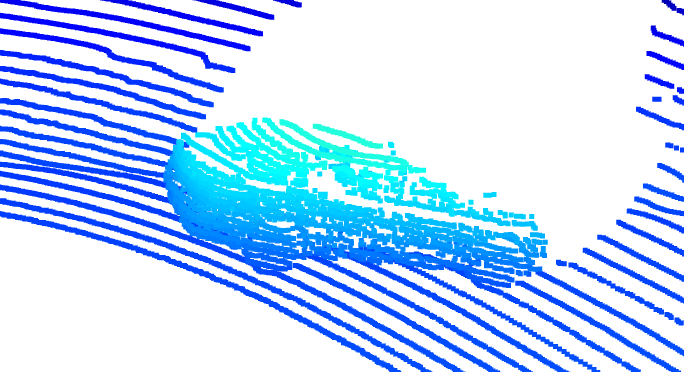
\includegraphics[scale=0.4]{../images_output/Seq1_Frame83.png}}
		\label{S1F83}
		\\
		\subfigure[Frame 91]{%
		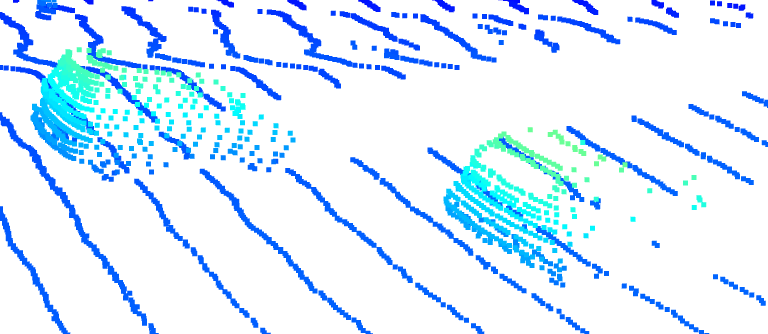
\includegraphics[scale=0.4]{../images_output/Seq1_Frame91.png}}
		\label{S1F91}
		\quad
		\subfigure[Sequence 1, Frame 124]{%
		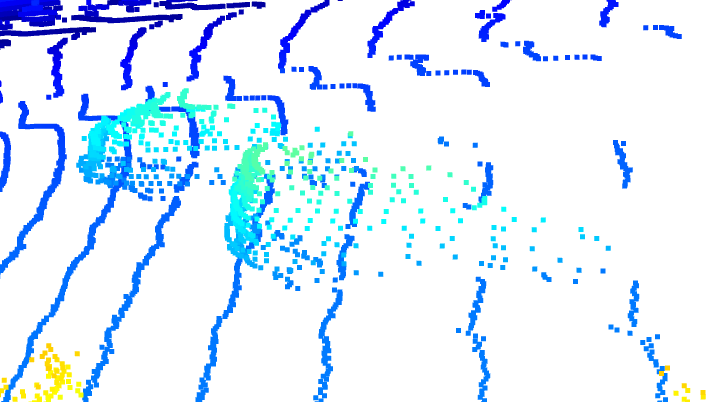
\includegraphics[scale=0.4]{../images_output/Seq1_Frame124.png}}
		\label{S1F124}
		%
		\caption{Sequence 1}
		\label{S1}
	\end{figure}
	
	\begin{figure}[H]
		\subfigure[Frame 3]{%
		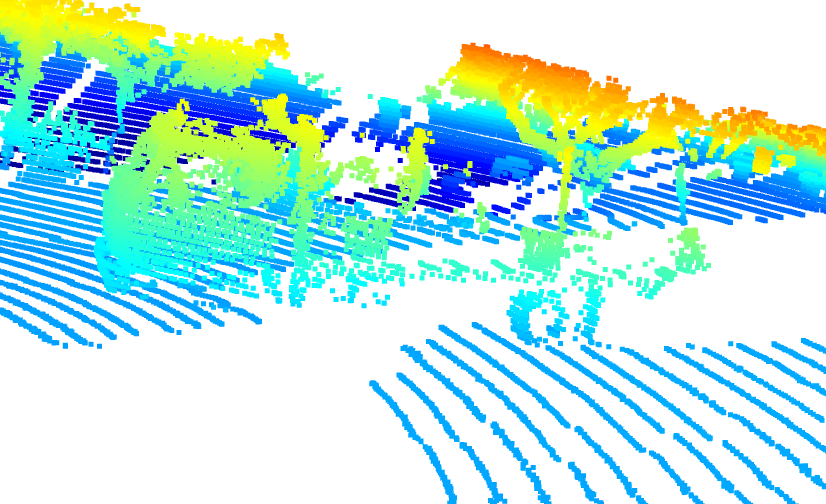
\includegraphics[scale=0.4]{../images_output/Seq2_Frame3.png}}
		\label{S2F3}
		\quad
		\subfigure[Frame 77]{%
		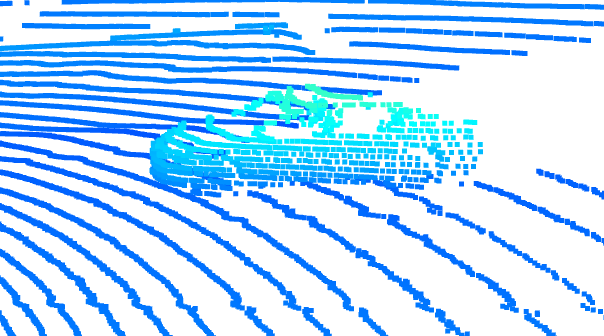
\includegraphics[scale=0.4]{../images_output/Seq2_Frame77.png}}
		\label{S2F77}
		\quad
		\subfigure[Frame 135]{%
		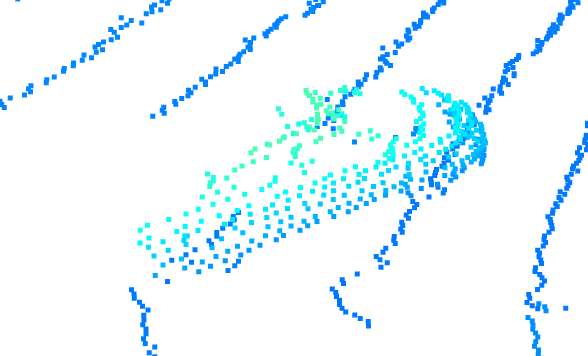
\includegraphics[scale=0.4]{../images_output/Seq2_Frame135.png}}
		\label{S2F135}
		%
		\caption{Sequence 2}
		\label{S2}
	\end{figure}
	
	\begin{figure}[H]
		\subfigure[Frame 2]{%
		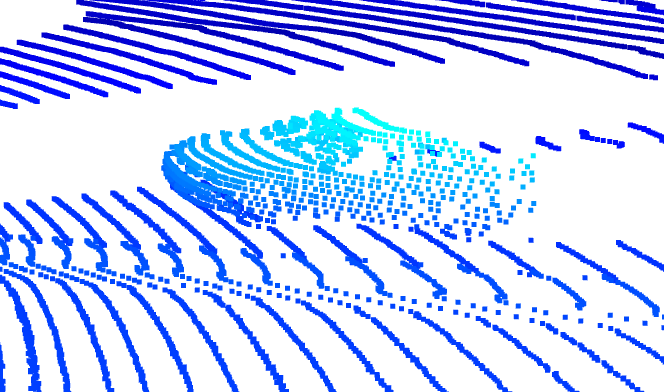
\includegraphics[scale=0.4]{../images_output/Seq3_Frame2.png}}
		\label{S3F2}
		\quad
		\subfigure[Frame 31]{%
		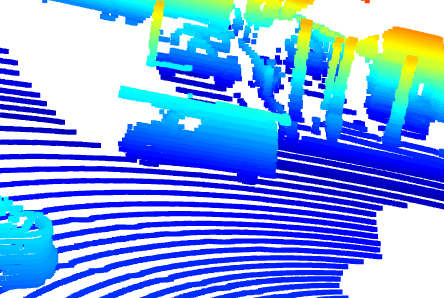
\includegraphics[scale=0.4]{../images_output/Seq3_Frame31.png}}
		\label{S3F31}
		\quad
		\subfigure[Frame 71]{%
		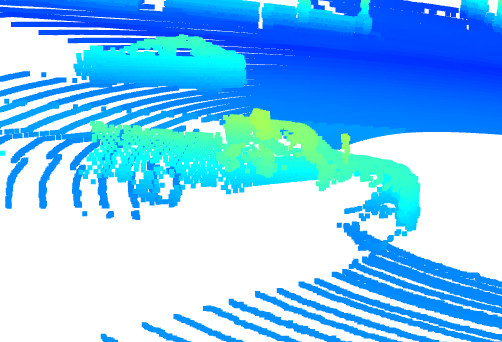
\includegraphics[scale=0.4]{../images_output/Seq3_Frame71.png}}
		\label{S3F71}
		\\
		\subfigure[Frame 108]{%
		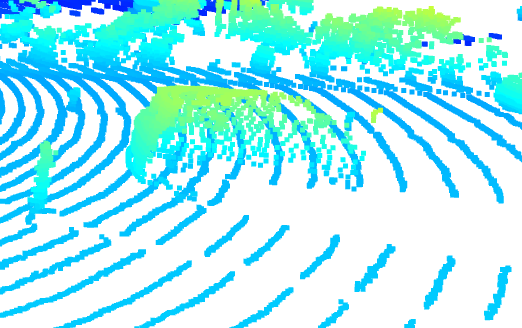
\includegraphics[scale=0.4]{../images_output/Seq3_Frame108.png}}
		\label{S3F108}
		\quad
		%
		\caption{Sequence 3}
		\label{S3}
	\end{figure}

	Examples of features which are visible in almost all images are:
	\begin{itemize}
		\item Tyres
		\item Roof
		\item Rear bumper (for cars in front)
		\item C-pillar (for cars in front)
		\item Hood (for cars behind)
		\item Windscreen (for cars behind)
		\item Front bumper (for cars behind)
		\item A-pillar (for cars behind)
	\end{itemize}



\end{document}
